\subsubsection{\stid{3.12} Sub-project: SUNDIALS}
\label{subsubsect:SUNDIALS-hypre}

\paragraph{Overview}

This project is enhancing the SUNDIALS library of numerical software packages
for evolving differential systems in time using state-of-the-art time
integration technologies for use on exascale systems.

The SUNDIALS suite of packages \cite{SUNDIALSweb} provides efficient and
adaptive time integrators and nonlinear solvers.  The packages are written using
encapsulation of both data structures and solvers, thus allowing easy
incorporation into existing codes and flexibility to take advantage of new
solver technologies and packages.  SUNDIALS provides both multistep and
multistage methods designed to evolve stiff or nonstiff ordinary (ODE) and
differential algebraic (DAE) systems with efficient accuracy-driven time step
selection.  SUNDIALS also provides both Newton and fixed point (with optional
acceleration) nonlinear solvers and scaled Krylov methods with hooks for
user-supplied preconditioners.  SUNDIALS is released with data structures and
interfaces to solvers supporting several programming environments, and users can
employ these supplied structures and interfaces or provide their own data
structures or solvers under the integrators.

Through software infrastructure developments, this project is enabling the
efficient and robust SUNDIALS time integrator packages to easily interoperate
with applications evolving time dependent systems as well as with external
linear and nonlinear solver packages developed for exascale computing.  In
addition, this project is providing support for integrating several independent
ordinary differential equation systems simultaneously on GPUs as part of
multiphysics applications.  Lastly, this project is supporting the deployment
and use of SUNDIALS packages within ECP applications, both through incorporation
into the discretization-based Co-Design Centers, AMReX and CEED, and directly
into applications.

\paragraph{Key Challenges}

Current implementations of efficient time integrators face challenges on many
fronts.  First, applications need both efficient integrators and ones that can
interface easily with efficient linear algebra packages to solve subservient
linear systems.  In addition, integrators and their interfaces to both solver
libraries and applications must be frequently updated to keep up with rapid
advances in system architectures. Some ECP applications require the solution of
many small systems of ODEs in parallel on GPUs giving rise to the specific need
for a GPU-enabled ODE time integration capability that can be used in parallel
for many systems at once and be able to run on multiple GPU-based architectures
with differing programming models.  Lastly, ECP applications require assistance
incorporating new linear solvers underneath the integrators and in updating
their interfaces to optimally use integrators on new platforms.


\paragraph{Solution Strategy}

This year, the SUNDIALS team will be performing regular performance assessments
of the SUNDIALS integrators within key ECP applications that use SUNDIALS,
including PeleC, PeleLM, and Nyx.  These assessments will involve running the
application codes on available early access hardware and evaluating SUNDIALS
performance, both due to systems aspects as well as algorithmic choices.

In addition, the SUNDIALS team will be working with the Pele team to assess a
new interface to the Ginkgo library of sparse linear solvers that will allow the
PeleLM and PelePhysics codes access to highly efficient solvers for batched
systems that work well on AMD GPUs.  This interface will provide additional
options to those available in the MAGMA solver library.  In addition, the
SUNDIALS team will evaluate the application of scaling factors for Jacobian
matrices supplied to direct linear solvers like MAGMA and Ginkgo.  These factors
have long been applied in the SUNDIALS use of iterative linear solvers, and they
drastically improve the numerical conditioning of the linear systems.

Also this year, the SUNDIALS team will evaluate the inclusion of mixed precision
linear solvers underneath its integrators.  While higher precision has generally
been necessary in time integrator algorithms due to the need to meet accuracy
tolerances, the linear solvers are used solely to update the solutions to the
nonlinear systems.  Hence these linear solvers can be fairly imprecise.  The
team will explore using the newest mixed precision solvers as a way to help
speed solutions on GPU-based systems.

Lastly, the SUNDIALS team is providing general support to ECP applications in
interfacing SUNDIALS packages into their software and in the optimal use of
advanced time integration algorithms.  This support will include working with
the application teams to help them install SUNDIALS, adjust their build systems
to appropriately link with the SUNDIALS library, choose the best algorithms for
their applications, and efficiently use (through parameter adjustments) the time
integrator methods in SUNDIALS.

\paragraph{Recent Progress}

SUNDIALS had four releases this past year, including new features in direct
support of ECP application needs.  In particular, releases in late 2020
delivered support for vectors, matrices, and solvers that make use of the HIP
programming model for use on AMD GPUs.  In addition, releases in spring and
summer of 2021 delivered similar support for the SYCL programming model for use
on Intel GPUs.  These new features are being used by the Pele and Nyx code
teams, and performance assessments are ongoing.

To support better performance evaluation within ECP applications, in FY21, the
SUNDIALS team implemented a new high performance test suite and performance
assessment layer.  The test suite consists of several short problems that can
scale to high numbers of unknowns and make use of a variety of programming
models and hybrid distributed parallel/GPU systems.  The test suite allows for
easier evaluation of performance on new platforms, including expected exascale
systems.  Moreover, the SUNDIALS team added a performance assessment layer and
enabled use of the ECP ST Caliper package for instrumentation underneath that
layer.  This year, the SUNDIALS team will conduct regular testing of this new
suite on EAS systems as a way of regularly updating build and install options
and improving library performance.

In fall of 2020, the SUNDIALS team completed initial assessments of performance
on AMD GPU systems \cite{balosEnablingGPUAccelerated2021} showing 5x speedups
using MPI+HIP over MPI+serial on advection-reaction problems using some of the
SUNDIALS advanced integrators.  In spring of 2021, the SUNDIALS team completed a
comprehensive study of the relative performance of several time integrators
within the PeleC application.  This study gave rise to new recommendations for
parameter settings that led to a 44\% reduction in runtime.

\begin{figure}[htb]
  \centering
  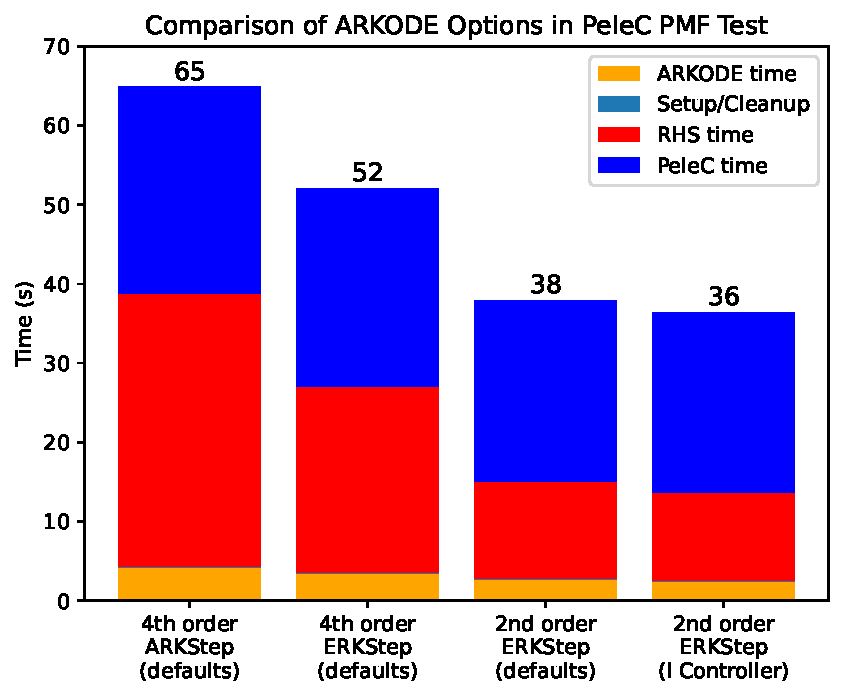
\includegraphics[width=0.6\linewidth]{projects/2.3.3-MathLibs/2.3.3.12-SUNDIALS-hypre/PeleC_fig.pdf}
  \caption{\label{fig:sun-many-demo} Runtimes from a pre-mixed flame test case
  in PeleC using various time integrators from SUNDIALS for chemistry evolution.
  Demonstrated 44\% reduction in runtime through algorithm choice using 2 nodes
  and 12 GPUs on Summit. Note that more efficient algorithms required fewer
  calls to the expensive right-hand-side function.}
\end{figure}

\paragraph{Early Access System Experiences}
The SUNDIALS team has been testing performance on both the Spock Early Access System and on the new Crusher system.  Figure \ref{fig:sun-spock-12-21} shows execution times for a 2D diffusion benchmark problem using the SUNDIALS CVODE integrator with a preconditioned conjugate gradient linear solver and run on one node of Spock using the new SUNDIALS profiling capabilities.  The maximum speedups (cpu time / gpu time) achieved are 3.8x, 3.9x, 2.1x, and 7.8x for the overall, linear solve, dot product, and right-hand-side times, respectively.  Furthermore, application partners with the PeleC, PeleLMeX, PelePhysics, Nyx, and MEUMAPPS-SS codes have all been able to run SUNDIALS within their codes on Spock. 

\begin{figure}[htb]
	\centering
	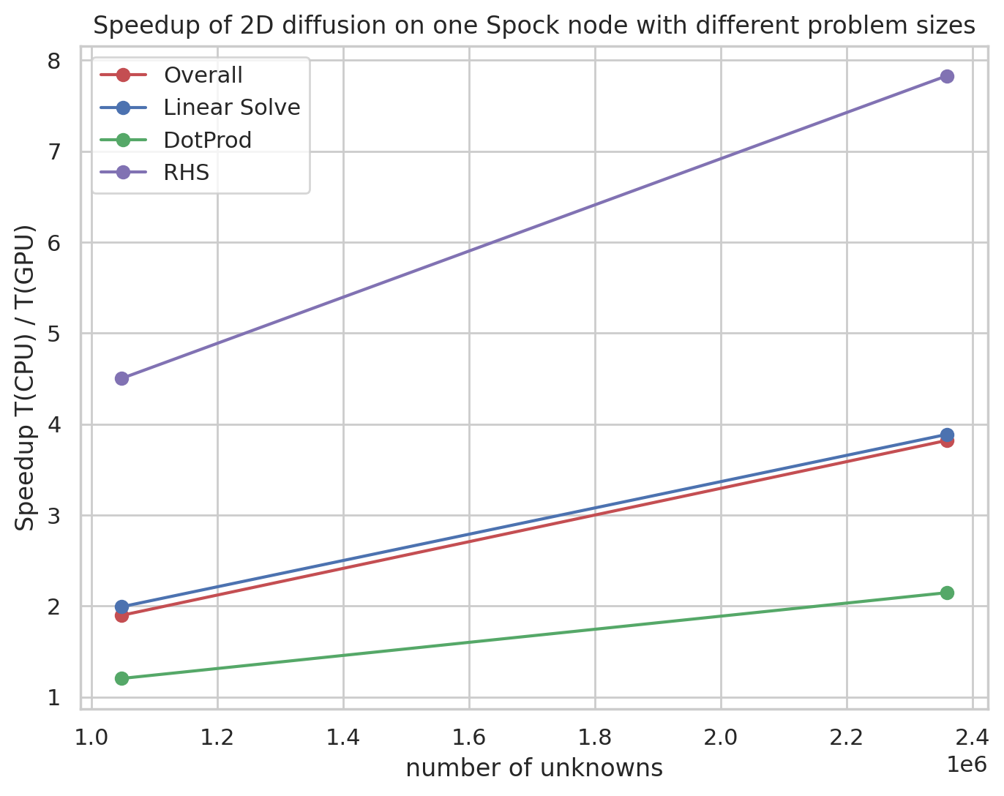
\includegraphics[width=0.6\linewidth]{projects/2.3.3-MathLibs/2.3.3.12-SUNDIALS-hypre/SpockResults-Dec2021.png}
%	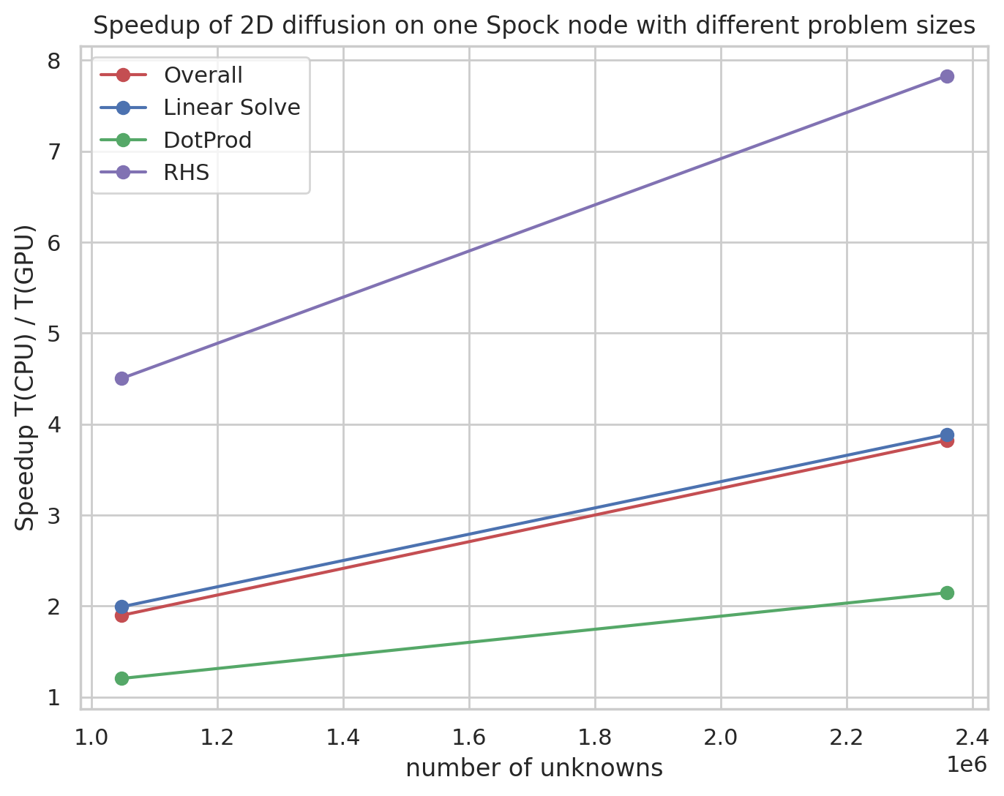
\includegraphics[width=0.6\linewidth]{projects/2.3.3-MathLibs/2.3.3.12-SUNDIALS-hypre/SpockResults-Dec2021.png}
	\caption{\label{fig:sun-spock-12-21} Speedup of 2D diffusion on one Spock node with differing problem sizes.  CPU problems used 60 CPU cores and GPU problems used all 4 MI100 GPUs on the node.}
\end{figure}

In addition, the SUNDIALS team recently ported to Crusher and executed the same 2D diffusion benchmark problem there using both the CVODE and ARKODE integrator packages.  
These results are in Figure \ref{fig:sun-crusher-spock-2-22}.
Running with problem sizes of $10^6$ and $10^7$, speedups of $\approx 1.53x$ for ARKODE and of $\approx 1.45x$ for CVODE were observed with Crusher over Spock ($T_{Spock} / T_{Crusher}).$  In addition, a speedup of $\approx 1.55x$ was observed for just the dot product operation.  These experiments used 1 MPI task with 1 MI100 GPU on Spock and 1 GCD of a MI250x GPU on Crusher.  Lastly, we note that the MEUMAPPS-SS (ExaAM project), PeleLMeX, and Nyx codes have successfully run using SUNDIALS on Crusher.

\begin{figure}[htb]
	\centering
	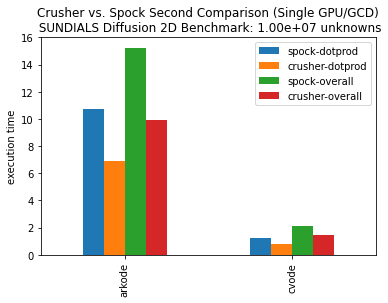
\includegraphics[width=0.6\linewidth]{projects/2.3.3-MathLibs/2.3.3.12-SUNDIALS-hypre/crusher-spock-1e7-Feb2022.png}
%	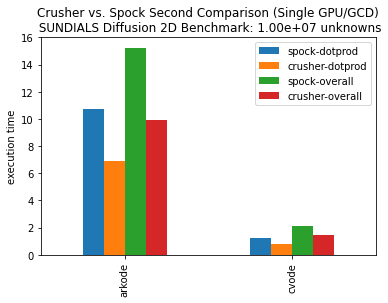
\includegraphics[width=0.6\linewidth]{projects/2.3.3-MathLibs/2.3.3.12-SUNDIALS-hypre/crusher-spock-1e7-Feb2022.png}
	\caption{\label{fig:sun-crusher-spock-2-22} Speedup of 2D diffusion with $10^7$ unknowns on 1 MPI task with 1 MI100 GPU on Spock and 1 GCD of a MI250x GPU on Crusher.}
\end{figure}

\paragraph{Next Steps}

During the remainder of FY22, this project team will:
\begin{enumerate}
  \item Perform regular assessments of SUNDIALS performance both with the new
        high performance test suite and within key applications on Early Access
        Systems.
  \item Implement new features in support of more efficient linear solves.
  \item Expand SUNDIALS support for Intel GPUs.
  \item Continue to support ECP applications in their use of SUNDIALS.
\end{enumerate}
